\section{Materialization and Reuse of Operations}\label{sec-materializaiton-and-reuse}
\todo[inline]{In this section, I only mention materialization for the feature engineering operations. I have some ideas for the model building operations as well, but I will skip that for now. If the ideas presented in this chapter are good enough for one complete paper, I can add my ideas for materialization and reuse of model building operations.}

Each operation on a data is mapped to an edge $e$ (representing the operation) that connects a vertex $v$ (representing the data) to another vertex $v'$ (representing the transformed data).
A series of operations on a data (a partial pipeline) are mapped to a path in the graph, starting from the vertex representing the data ($v$), along an ordered list of edges, each representing one operation ($e_i$), resulting in the final data ($v'$). 
Each edge in the path connects the source data ($v_i$) to a intermediate transformed data ($v_{i+1}$).
Using this representation, we can search the graph constructed from the experiment database to look for reuse opportunities.

Algorithm \ref{alg-reuse} shows the process of detecting reuse for one operation.
\begin{algorithm}
\caption{Reuse algorithm}\label{alg-reuse}
\begin{algorithmic}[1]
\Require vertex $d$ (dataset), edge $e$ (transformation), graph $G$ (experiment graph)
\Ensure vertex $d'$ representing the transformed data (returns the input vertex if reuse is not possible)
\Function{Reuse}{$d,e,G$}
	\If {$d \in G$}
		\For {$i$ in $out\_edges(G,d)$}
			 	\If {$i = e$} \Comment{the transformation exists}
			 		 \State \textbf{return} $i.destination$ 
			 	\EndIf
		\EndFor
	\EndIf
   \State \textbf{return} $d$ \Comment{return the source dataset if reuse is not possible}
\EndFunction
\end{algorithmic}
\end{algorithm}

 
\begin{algorithm}
\caption{Path Reuse algorithm}\label{alg-reuse-partial_pipeline}
\begin{algorithmic}[1]
\Require vertex $d$ (dataset), edge list $E$ (transformations), graph $G$ (experiment graph)
\Ensure vertex $d'$ representing the transformed data to use
\Function{Reuse\_path}{$d,E,G$}
	\State $next$ = $REUSE(d, E[0],G)$
	\If {$next = d$}
		\State \textbf{return} $next$
	\ElsIf {$E.size > 1$}
		\State \textbf{return} $REUSE\_PATH(next, E - E[0], G)$
	\Else
		\State \textbf{return} $next$
	\EndIf
\EndFunction
\end{algorithmic}
\end{algorithm}
 
Algorithm \ref{alg-reuse-partial_pipeline} shows the process of detecting reuse opportunities for a path.
When reuse is possible, the Function $REUSE\_PATH$ returns the transformed dataset closest to the end of the path, thus, skipping as many transformations as possible.

\subsection{The Problem of Unaligned Pipelines}
The reuse algorithms (Algorithms \ref{alg-reuse} and \ref{alg-reuse-partial_pipeline}) have one drawback that affects real-world use cases.
In our analysis of the Kaggle scripts, we realize that although large parts of the operations are the same across multiple notebooks, sometimes there are slight differences.
There are two common problematic scenarios that occur when users are writing scripts.
First, users tend to apply the operations in arbitrary order and while the final results may be the same the process of arriving at the result is different.
Second, users tend to enhance other user's script by adding their own operations to the data processing pipeline.
However, our analysis shows that many of the custom or reordered operations are applied to different columns and thus they are not affecting each other.

Figure \ref{fig-unaligned-operations} shows the two problematic scenarios that may occur.
Although in both scenarios the operations can be reused, the Algorithms \ref{alg-reuse} and \ref{alg-reuse-partial_pipeline} are not able to detect them as the vertices in the transformations are different. 
The experiment graph consists of the original training dataset, and 4 operations, where $oper\_1$, $oper\_2$, and $oper\_3$ transform different columns.
In scenario 1, the user performs two transformations and then transforms the resulting data using $oper\_1$, $oper\_2$, and $oper\_3$.
In scenario 2, the same transformations ($oper\_1$, $oper\_2$, and $oper\_3$) are applied to the training data.
However, the order of the transformations is different.
Simple reuse algorithms (Algorithms \ref{alg-reuse}, \ref{alg-reuse-partial_pipeline}) are not able to detect the reuse opportunities in these two scenarios.

\begin{figure}
\centering
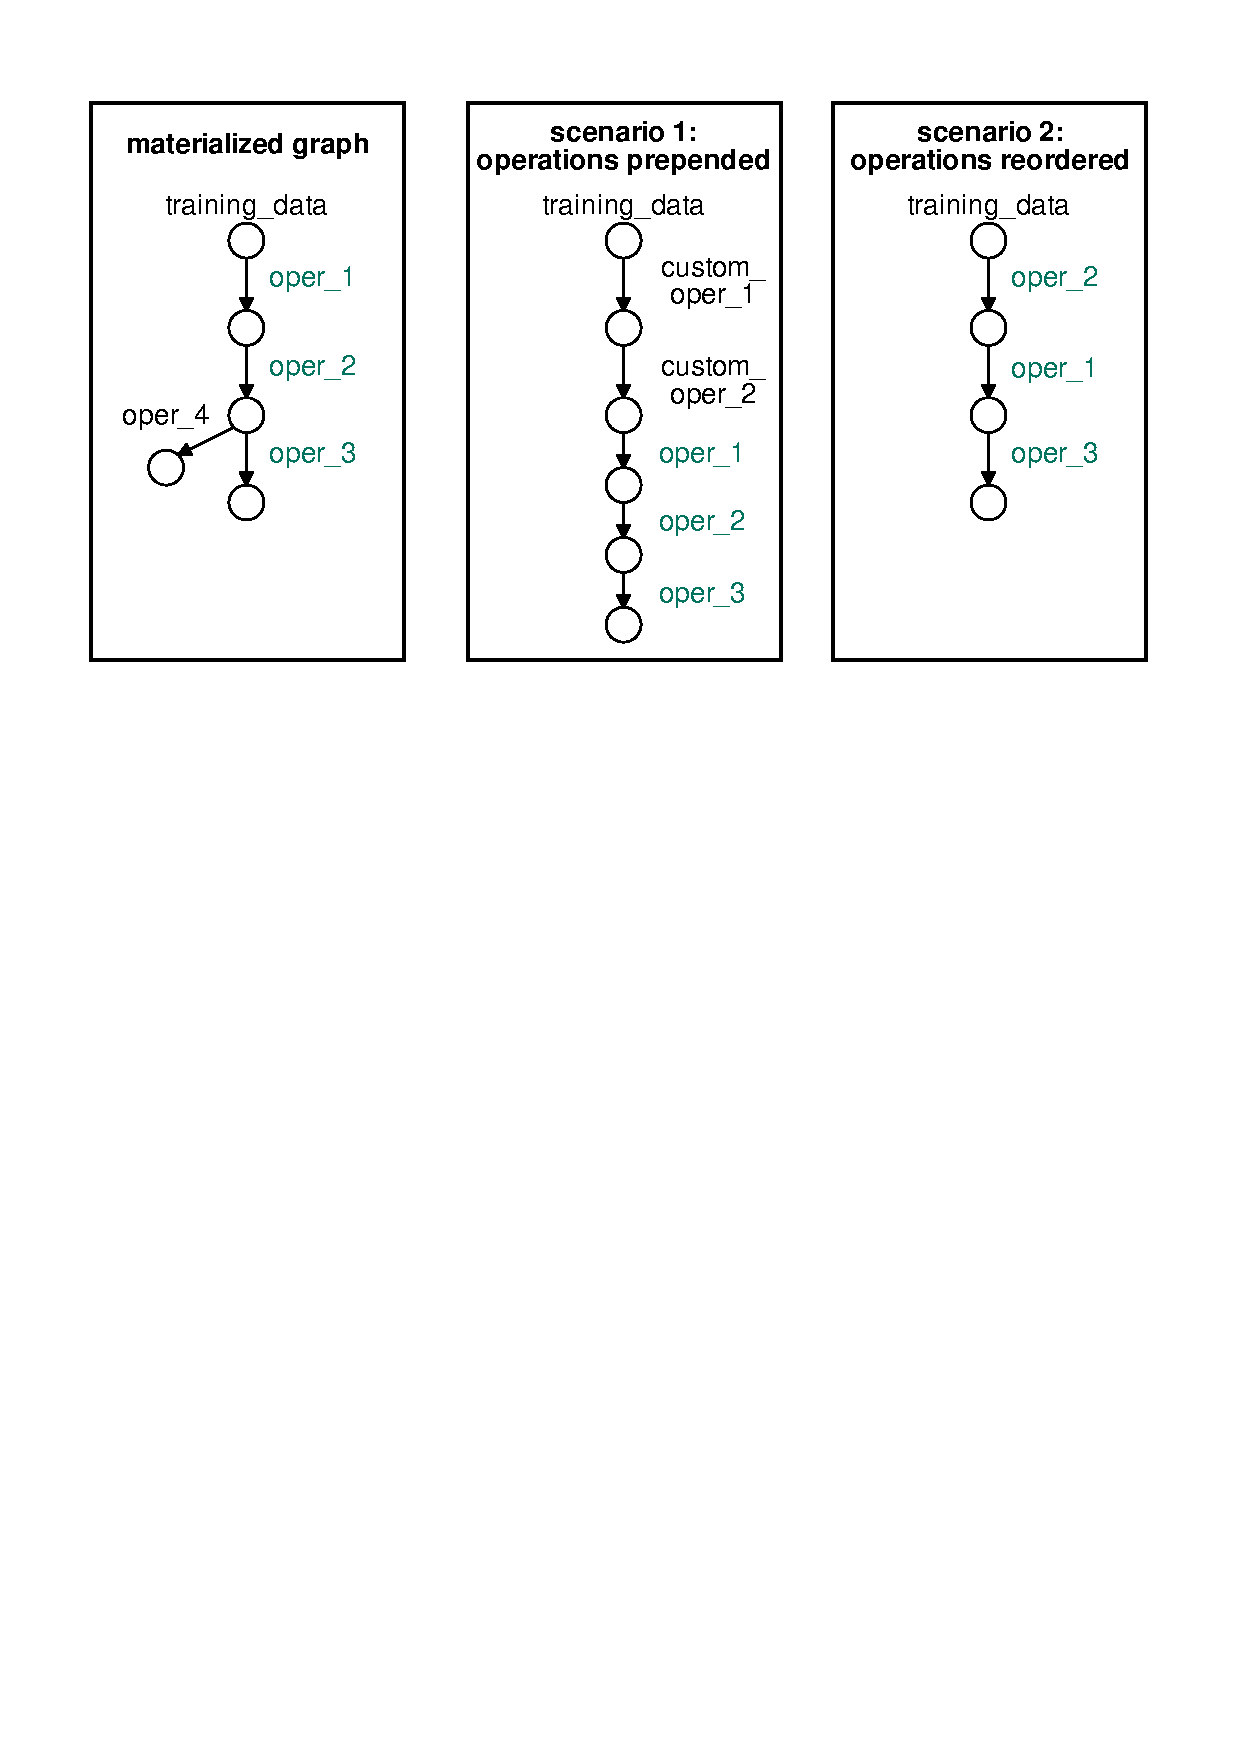
\includegraphics[width=\columnwidth]{../images/unaligned-operations}
\caption{Two scenarios that direct reuse cannot be applied}
\label{fig-unaligned-operations}
\end{figure}

To apply reuse in these scenarios we have to augment the experiment graph to capture such mutual-exclusive transformations.

\subsection{Augmented Experiment Graph}
In this section, we explain our approach for augmenting the graph $G$, constructed from the experiment database, to capture the operations that are order-independent.
The augmented graph enables our reuse algorithms to detect reuse opportunities in presence of prepended and reordered operations.
Algorithms \ref{alg-add-augment-graph} and \ref{alg-augment-graph} shows the process of adding and augmenting the graph given a new transformation.
We augment the graph $G$ with edges that connect vertices (datasets) that can be derived from earlier vertices using the same transformation.
When a new transformation is added, the graph is traversed in the opposite direction of the edges starting from the current vertex (source of the transformation).
If the preceding vertices contain all the columns involved in the transformation (i.e. \textit{i\_columns}), an edge is added to the graph.
The process continues until a vertex does not contain all the input columns, or the traversal reaches the root vertex (i.e., $in\_edges(G,d) = \emptyset$).

\begin{algorithm}
\caption{Add and Augment Graph algorithm}\label{alg-add-augment-graph}
\begin{algorithmic}[1]
\Require vertex $d$ (dataset), edge $e$ (transformation), graph $G$ (experiment graph)
\Ensure Graph $G$ containing the new transformation and all the augment edges
\Function{Add\_And\_Augment\_Graph}{$d,e,G$}
	\State $G = G.add\_edge(e)$ \Comment{Add the transformation to the graph}
	\State $destination = e.destination$ 
	\State $tf=e.tf$ 
	\State $ic=e.in\_columns$ \Comment{columns involved in e}
	\State \textbf{return} $AUGMENT\_GRAPH(d, destination,ic, tf, G)$   \Comment{Call the recursive augment procedure}
\EndFunction
\end{algorithmic}
\end{algorithm}

\begin{algorithm}
\caption{Augment Graph algorithm}\label{alg-augment-graph}
\begin{algorithmic}[1]
\Require vertex $d$ (dataset), vertex $d'$ (transformed dataset), input columns $ic$ (of the transformations), transformation function $tf$, graph $G$ (experiment graph)
\Ensure Graph $G$ representing the augmented graph
\Function{Augment\_Graph}{$d,d',ic,tf,G$}
	\For {$p$ in $parents_of(G,d)$ }
		\If {$p.columns.contains(ic)$}
			\State  $new\_edge=Edge(p, d', ic,tf)$
			\State $G = G.add\_edge(new\_edge)$
			\State  $AUGMENT\_GRAPH(p, d',ic, tf,G)$
		\EndIf
	\EndFor
   \State \textbf{return} $G$
\EndFunction
\end{algorithmic}
\end{algorithm}


Figure \ref{fig-augmented-graph} shows the augmented graph of Figure \ref{fig-unaligned-operations}.
Using the augmented graph, the reuse algorithms can detect reuse opportunities for both scenarios (operations prepended and operations reordered).

\begin{figure}
\centering
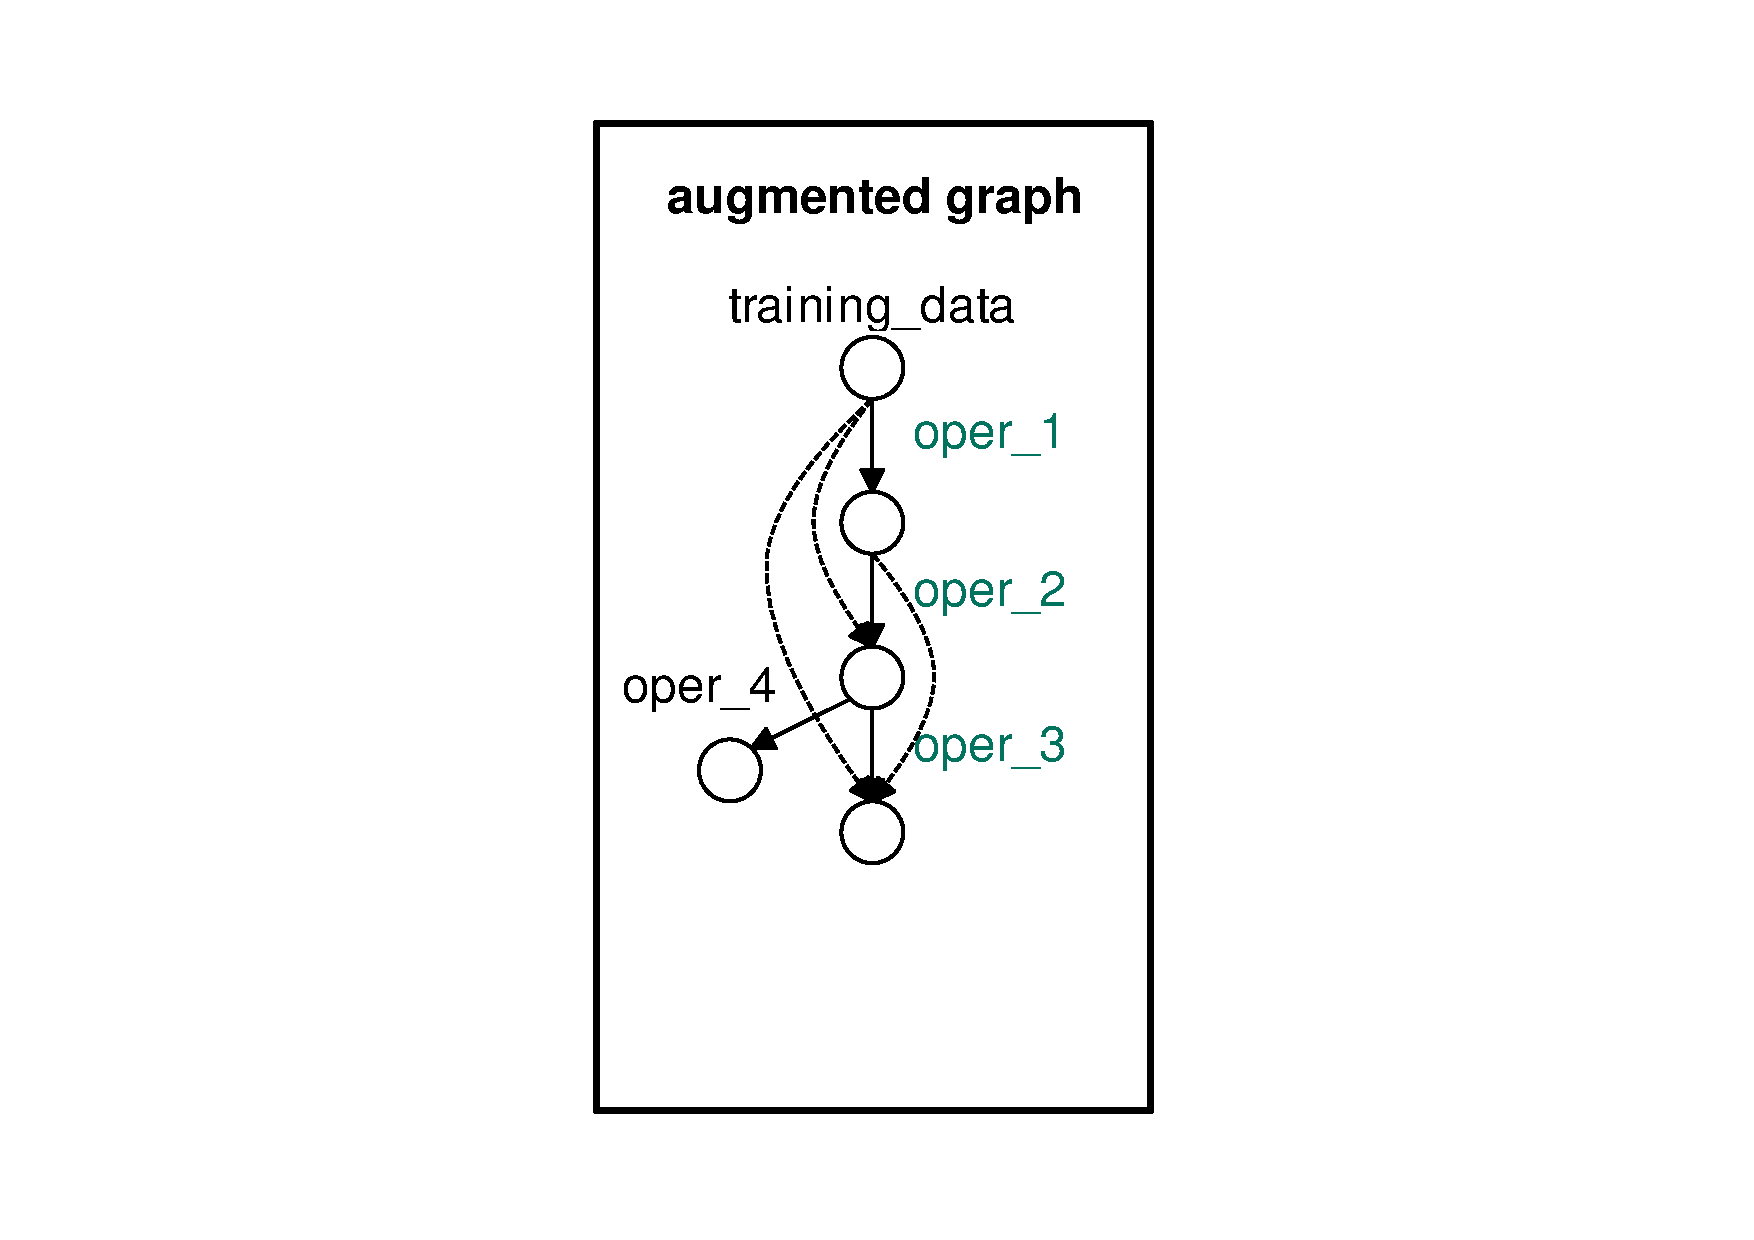
\includegraphics[width=0.33\columnwidth]{../images/augmented-graph}
\caption{Augmented graph from Figure \ref{fig-unaligned-operations} }
\label{fig-augmented-graph}
\end{figure}

%\subsection{Materialization of Grid Search}
%\todo[inline]{Incomplete}
%In order to analyze whether or not we should materialize parts of the grid search, we first have to unpack it, and compare it with other grid search.
%Then, similar to Section \ref{sub-sec-materialization-of-transformed-data}, we materialize the parts that are executed frequently.
%
%%\subsection{Guided Grid-Search}
%%\todo[inline]{just an idea}
%%By extracting correlation between different parameters and the model quality we can provided a guided grid search, where we can provide some estimate or show the effects of a hyperparameter range on the model quality